% !TEX spellcheck = en_US



% ~~~~~~~~~~~~~~~~~~~~~~~~~~~~~~~~~~~~~~~ V
% (NC) 2026 Haluk Bingol
% github.com/halukbingol/LaTeX-Templates
%
% Licensees may copy, distribute, display, and perform the work and make derivative works 
% and remixes based on it only for non-commercial purposes. 
% ~~~~~~~~~~~~~~~~~~~~~~~~~~~~~~~~~~~~~~~ A




% =====================================================================
%  Strings in Java -- The Concepts
%  ---------------------------------------------------------------------
%  Built on hbCisLaTeXTemplate.tex with the libraries in ../../hblib/.
%  Programs and their outputs are read from codeoutput/:
%     codeoutput/<Name>.java   the program
%     codeoutput/<Name>.in     keyboard input (optional)
%     codeoutput/<Name>.txt    what it printed, made by:  sh run_examples.sh
% =====================================================================

\documentclass[aspectratio=169,10pt,compress]{beamer}

% ~~~~~~~~~~~~~~~~~~~~~~~~~~~~~~~~~~~~~~~~~~~~~~~~~~~~~~~~~~~~~~~~~ V hblib
	\usepackage{../../hblib/hblibPresentation} % lib presentation: theme, i/N, \hSection, algorithm2e, ...
	\usepackage{../../hblib/hblibCodeoutput} % lib code + output: \lstcode, \lstcodedown, ...
	\usepackage{../../hblib/hblibDatastructures} % lib data structures: \hString, \hStack, \hQueue
% ~~~~~~~~~~~~~~~~~~~~~~~~~~~~~~~~~~~~~~~~~~~~~~~~~~~~~~~~~~~~~~~~~ A hblib


% xcolor, array (and the L{width} column), listings, tikz and algorithm2e come from the hblib libraries
\usepackage[T1]{fontenc}
\usepackage{lmodern}
\usepackage{booktabs}

\definecolor{gitred}{RGB}{240,80,50}
\newcommand{\cmd}[1]{\texttt{\color{gitred}#1}}

\usetikzlibrary{fit}
\tikzset{
  var/.style={draw, thick, fill=blue!8, minimum width=1.1cm, minimum height=0.55cm, font=\ttfamily\small},
  obj/.style={draw, thick, rounded corners, fill=orange!10, inner sep=4pt},
  objfit/.style={draw, thick, rounded corners, orange!70!black, inner sep=0pt},
  ref/.style={-{Stealth[length=2.5mm]}, thick, blue!60!black},
  lbl/.style={font=\scriptsize\sffamily, text=gray!70!black}
}

% ---------------------------------------------------------------------
\title{Strings in Java}
\subtitle{The Concepts}
\author[Bingol]{Haluk O. Bingol}

\institute[FCIS]{
    Faculty of Computer and Information Sciences\\
    Yeditepe University
}
\date{
	{\tiny \hbTimeStamp}
}

\begin{document}




% ~~~~~~~~~~~~~~~~~~~~~~~~~~~~~~~~~~~~~~ V frm
\begin{frame}[t,fragile]
  \titlepage
\end{frame}
% ~~~~~~~~~~~~~~~~~~~~~~~~~~~~~~~~~~~~~~ A frm




% ~~~~~~~~~~~~~~~~~~~~~~~~~~~~~~~~~~~~~~ V frm
\begin{frame}[t,fragile] \frametitle{Outline}
  \tableofcontents[hideallsubsections]
\end{frame}
% ~~~~~~~~~~~~~~~~~~~~~~~~~~~~~~~~~~~~~~ A frm

% ~~~~~~~~~~~~~~~~~~~~~~~~~~~~~~~~~~~~~~ V
\hSection[What]{What Is a String?}{}{}
% ~~~~~~~~~~~~~~~~~~~~~~~~~~~~~~~~~~~~~~ A

% ~~~~~~~~~~~~~~~~~~~~~~~~~~~~~~~~~~~~~~ V
\subsection[Text]{Text in programs}
% ~~~~~~~~~~~~~~~~~~~~~~~~~~~~~~~~~~~~~~ A




% ~~~~~~~~~~~~~~~~~~~~~~~~~~~~~~~~~~~~~~ V frm
\begin{frame}[t,fragile] \frametitle{Text is everywhere}
  \begin{columns}[T]
    \begin{column}{0.48\textwidth}
      Programs handle text all the time:
      \begin{itemize}\small
        \item names, addresses, messages
        \item commands typed by a user
        \item file and web page contents
        \item DNA sequences: \texttt{GATTACA}
        \item source code itself
      \end{itemize}
      \begin{block}{Definition}
        \small A \textbf{string} is a finite sequence of \textbf{characters}.
        Its \textbf{length} is the number of characters.
      \end{block}
    \end{column}
    \begin{column}{0.48\textwidth}
      The string \texttt{"Hello, World"} has length 12:
      \vspace{0.6em}

      \begin{tikzpicture}\hString[0.42]{H,e,l,l,o,{,},\textvisiblespace,W,o,r,l,d}\end{tikzpicture}

      \vspace{0.6em}
      \small Each character has a \textbf{position} (index), starting at \textbf{0}.
      The space and the comma are characters too.

      \vspace{0.4em}
      The \textbf{empty string} \texttt{""} has length 0.
    \end{column}
  \end{columns}
\end{frame}
% ~~~~~~~~~~~~~~~~~~~~~~~~~~~~~~~~~~~~~~ A frm




% ~~~~~~~~~~~~~~~~~~~~~~~~~~~~~~~~~~~~~~ V frm
\begin{frame}[t,fragile] \frametitle{A character and a string are different things}
  \small
  \begin{tabular}{@{}L{0.22\textwidth}L{0.33\textwidth}L{0.36\textwidth}@{}}
    \toprule
                       & \textbf{\texttt{char}}                  & \textbf{\texttt{String}} \\
    \midrule
    holds              & exactly \textbf{one} character           & \textbf{zero or more} characters \\
    literal            & single quotes: \texttt{'A'}              & double quotes: \texttt{"A"}, \texttt{""}, \texttt{"Ali"} \\
    kind of type       & \textbf{primitive} (a 16-bit number)     & \textbf{class} (objects, with methods) \\
    stored             & the value itself                          & a \textbf{reference} to an object \\
    default value      & \texttt{'\textbackslash u0000'}          & \texttt{null} (no object) \\
    compare with       & \texttt{==}                               & \texttt{equals(...)} \\
    \bottomrule
  \end{tabular}

  \vspace{0.8em}
  \begin{alertblock}{\texttt{'A'} is not \texttt{"A"}}
    \texttt{'A'} is the number 65 in disguise. \texttt{"A"} is an object that \emph{contains} one character.
    Mixing them up is one of the most common beginner errors.
  \end{alertblock}
\end{frame}
% ~~~~~~~~~~~~~~~~~~~~~~~~~~~~~~~~~~~~~~ A frm

% ~~~~~~~~~~~~~~~~~~~~~~~~~~~~~~~~~~~~~~ V
\hSection[Objects]{Strings Are Objects}{}{}
% ~~~~~~~~~~~~~~~~~~~~~~~~~~~~~~~~~~~~~~ A

% ~~~~~~~~~~~~~~~~~~~~~~~~~~~~~~~~~~~~~~ V
\subsection[Reference]{Variables hold references}
% ~~~~~~~~~~~~~~~~~~~~~~~~~~~~~~~~~~~~~~ A




% ~~~~~~~~~~~~~~~~~~~~~~~~~~~~~~~~~~~~~~ V frm
\begin{frame}[t,fragile] \frametitle{A variable holds a reference}
  \begin{columns}[T]
    \begin{column}{0.5\textwidth}


% +++++++++++++++++++++++++++++++++++++++ V lst
%: -Lst.
\begin{lstlisting}[style=codesnippet, language=Java]
String s = "Hello";
int    n = s.length();    // 5
char   c = s.charAt(1);   // 'e'
\end{lstlisting}
% +++++++++++++++++++++++++++++++++++++++ A lst



      \begin{itemize}\small
        \item \texttt{s} does not contain the letters; it \textbf{refers} (points) to a \texttt{String} object
        \item We \textbf{ask the object}: \texttt{s.length()}, \texttt{s.charAt(1)}
        \item The object knows its characters and offers about 70 methods
      \end{itemize}
    \end{column}
    \begin{column}{0.46\textwidth}
      \begin{center}
      \begin{tikzpicture}
        \node[var] (s) at (0,0) {s};
        \node[lbl, above=1pt of s] {variable};
\begin{scope}[shift={(2.2,-0.200)}]\hString[0.4]{H,e,l,l,o}\end{scope}
\node[objfit, fit={(2.080,-0.320) (4.320,0.500)}] (o) {};

        \node[lbl, above=1pt of o] {String object};
        \draw[ref] (s) -- (o);
        \node[var] (n) at (0,-1.4) {5};
        \node[lbl, left=2pt of n] {\texttt{n}};
        \node[var] (c) at (0,-2.3) {'e'};
        \node[lbl, left=2pt of c] {\texttt{c}};
        \node[lbl, align=left, anchor=west] at (1.2,-1.85) {primitives:\\the value itself};
      \end{tikzpicture}
      \end{center}
    \end{column}
  \end{columns}
\end{frame}
% ~~~~~~~~~~~~~~~~~~~~~~~~~~~~~~~~~~~~~~ A frm

% ~~~~~~~~~~~~~~~~~~~~~~~~~~~~~~~~~~~~~~ V
\subsection[Index]{Positions and pieces}
% ~~~~~~~~~~~~~~~~~~~~~~~~~~~~~~~~~~~~~~ A




% ~~~~~~~~~~~~~~~~~~~~~~~~~~~~~~~~~~~~~~ V frm
\begin{frame}[t,fragile] \frametitle{Positions start at 0}
  \begin{center}
    \begin{tikzpicture}\hString[0.55]{Y,e,d,i,t,e,p,e}[4][8]\end{tikzpicture}
  \end{center}
  \vspace{0.3em}
  \small
  \begin{tabular}{@{}L{0.34\textwidth}L{0.18\textwidth}L{0.4\textwidth}@{}}
    \toprule
    \textbf{Expression}            & \textbf{Value}       & \textbf{Why} \\
    \midrule
    \texttt{s.length()}            & \texttt{8}           & 8 characters \\
    \texttt{s.charAt(0)}           & \texttt{'Y'}         & first index is 0 \\
    \texttt{s.charAt(s.length()-1)}& \texttt{'e'}         & last index is \texttt{length-1} \\
    \texttt{s.substring(4, 8)}     & \texttt{"tepe"}      & from 4 \textbf{up to, not including}, 8 (highlighted) \\
    \texttt{s.indexOf("tepe")}     & \texttt{4}           & where it starts; \texttt{-1} if not found \\
    \texttt{s.charAt(8)}           & \emph{exception}     & index 8 does not exist \\
    \bottomrule
  \end{tabular}

  \vspace{0.4em}
  \hRemark{Rule of thumb:} \texttt{substring(b, e)} has length \texttt{e - b}.
\end{frame}
% ~~~~~~~~~~~~~~~~~~~~~~~~~~~~~~~~~~~~~~ A frm




% ~~~~~~~~~~~~~~~~~~~~~~~~~~~~~~~~~~~~~~ V frm
\begin{frame}[t,fragile] \frametitle{Nothing, empty, or blank?}
  \begin{columns}[T]
    \begin{column}{0.5\textwidth}
      \begin{center}
      \begin{tikzpicture}
        \node[var] (a) at (0,0) {a};
        \node[font=\ttfamily\small, anchor=west] at (1.0,0) {null \quad (no object)};
        \node[var] (b) at (0,-1.3) {b};
\node[objfit, minimum width=0.5cm, minimum height=0.5cm] (ob) at (1.65,-1.3) {};

        \node[lbl, right=2pt of ob] {length 0};
        \draw[ref] (b) -- (ob);
        \node[var] (c) at (0,-2.6) {c};
\begin{scope}[shift={(1.4,-2.800)}]\hString[0.4]{\textvisiblespace,\textvisiblespace,\textvisiblespace}\end{scope}
\node[objfit, fit={(1.280,-2.920) (2.720,-2.100)}] (oc) {};

        \node[lbl, right=2pt of oc] {length 3};
        \draw[ref] (c) -- (oc);
      \end{tikzpicture}
      \end{center}


% +++++++++++++++++++++++++++++++++++++++ V lst
%: -Lst.
\begin{lstlisting}[style=codesnippet, language=Java]
String a = null;
String b = "";
String c = "   ";
\end{lstlisting}
% +++++++++++++++++++++++++++++++++++++++ A lst



    \end{column}
    \begin{column}{0.46\textwidth}
      \small
      \begin{tabular}{@{}lccc@{}}
        \toprule
                               & \texttt{a}     & \texttt{b}    & \texttt{c} \\
        \midrule
        \texttt{x == null}     & true           & false         & false \\
        \texttt{x.isEmpty()}   & \emph{error}   & true          & false \\
        \texttt{x.isBlank()}   & \emph{error}   & true          & true \\
        \bottomrule
      \end{tabular}

      \vspace{0.6em}
      \begin{alertblock}{NullPointerException}
        \small Calling a method on \texttt{null} fails: there is no object to ask.
        Check \texttt{x != null} first, or write \texttt{"text".equals(x)}.
      \end{alertblock}
    \end{column}
  \end{columns}
\end{frame}
% ~~~~~~~~~~~~~~~~~~~~~~~~~~~~~~~~~~~~~~ A frm

% ~~~~~~~~~~~~~~~~~~~~~~~~~~~~~~~~~~~~~~ V
\hSection[Immutable]{Immutability}{}{}
% ~~~~~~~~~~~~~~~~~~~~~~~~~~~~~~~~~~~~~~ A

% ~~~~~~~~~~~~~~~~~~~~~~~~~~~~~~~~~~~~~~ V
\subsection[Never]{A String never changes}
% ~~~~~~~~~~~~~~~~~~~~~~~~~~~~~~~~~~~~~~ A




% ~~~~~~~~~~~~~~~~~~~~~~~~~~~~~~~~~~~~~~ V frm
\begin{frame}[t,fragile] \frametitle{A String never changes}
  \begin{columns}[T]
    \begin{column}{0.44\textwidth}


% +++++++++++++++++++++++++++++++++++++++ V lst
%: -Lst.
\begin{lstlisting}[style=codesnippet, language=Java]
String s = "java";
s.toUpperCase();      // result lost!
s = s.toUpperCase();  // s now refers
                      // to a new object
\end{lstlisting}
% +++++++++++++++++++++++++++++++++++++++ A lst



      \begin{itemize}\small
        \item Every ``changing'' method (\texttt{toUpperCase}, \texttt{replace}, \texttt{trim}, \dots)
              \textbf{returns a new} \texttt{String}
        \item The original object is never modified
        \item An object nobody refers to is removed by the \textbf{garbage collector}
      \end{itemize}
    \end{column}
    \begin{column}{0.52\textwidth}
      \begin{center}
      \begin{tikzpicture}
        \node[lbl] at (1.5,0.9) {before \texttt{s = s.toUpperCase();}};
        \node[var] (s1) at (0,0) {s};
\begin{scope}[shift={(1.6,-0.200)}]\hString[0.4]{j,a,v,a}\end{scope}
\node[objfit, fit={(1.480,-0.320) (3.320,0.500)}] (o1) {};

        \draw[ref] (s1) -- (o1);

        \node[lbl] at (0,-1.3) {after};
        \node[var] (s2) at (0,-2.0) {s};
        \begin{scope}[opacity=0.4]
\begin{scope}[shift={(1.6,-1.800)}]\hString[0.4]{j,a,v,a}\end{scope}
\node[objfit, fit={(1.480,-1.920) (3.320,-1.100)}] (o2) {};

        \end{scope}
\begin{scope}[shift={(1.6,-3.000)}]\hString[0.4]{J,A,V,A}[0][4]\end{scope}
\node[objfit, fit={(1.480,-3.120) (3.320,-2.300)}] (o3) {};

        \draw[ref] (s2) -- (o3.west);
        \node[lbl, right=2pt of o2, align=left] {unchanged,\\garbage now};
        \node[lbl, right=2pt of o3] {new object};
      \end{tikzpicture}
      \end{center}
    \end{column}
  \end{columns}
\end{frame}
% ~~~~~~~~~~~~~~~~~~~~~~~~~~~~~~~~~~~~~~ A frm




% ~~~~~~~~~~~~~~~~~~~~~~~~~~~~~~~~~~~~~~ V frm
\begin{frame}[t,fragile] \frametitle{Why are strings immutable?}
  \begin{columns}[T]
    \begin{column}{0.48\textwidth}
      \begin{block}{Safe sharing}
        \small Many variables can refer to the same string. Nobody can change it under the others' feet.
      \end{block}
      \begin{block}{Security}
        \small A file name or URL checked once cannot be altered after the check.
      \end{block}
      \begin{block}{Threads}
        \small Immutable objects can be used by many threads without locks.
      \end{block}
    \end{column}
    \begin{column}{0.48\textwidth}
      \begin{block}{Hashing}
        \small Strings are the most common \texttt{HashMap} keys. Their hash code never changes,
        so it is computed once and cached.
      \end{block}
      \begin{block}{The string pool}
        \small Equal literals can share one object, saving memory (next section).
      \end{block}
      \begin{alertblock}{The price}
        \small Building a long string piece by piece creates many temporary objects.
        That is what \texttt{StringBuilder} is for.
      \end{alertblock}
    \end{column}
  \end{columns}
\end{frame}
% ~~~~~~~~~~~~~~~~~~~~~~~~~~~~~~~~~~~~~~ A frm

% ~~~~~~~~~~~~~~~~~~~~~~~~~~~~~~~~~~~~~~ V
\subsection[Builder]{Building strings}
% ~~~~~~~~~~~~~~~~~~~~~~~~~~~~~~~~~~~~~~ A




% ~~~~~~~~~~~~~~~~~~~~~~~~~~~~~~~~~~~~~~ V frm
\begin{frame}[t,fragile] \frametitle{Building a string: \texttt{+} versus \texttt{StringBuilder}}
  \begin{columns}[T]
    \begin{column}{0.48\textwidth}


% +++++++++++++++++++++++++++++++++++++++ V lst
%: -Lst.
\begin{lstlisting}[style=codesnippet, language=Java]
String s = "";
for (int i = 0; i < n; i++)
    s = s + "x";    // new object each time
\end{lstlisting}
% +++++++++++++++++++++++++++++++++++++++ A lst



      \small Step $k$ copies the $k$ characters built so far into a new object. In total:
      \[
      	1 + 2 + \dots + n = \frac{n(n+1)}{2} \in O(n^{2})
      \]
      \small For $n = 100\,000$ that is about 5 billion copied characters.
    \end{column}
    \begin{column}{0.48\textwidth}


% +++++++++++++++++++++++++++++++++++++++ V lst
%: -Lst.
\begin{lstlisting}[style=codesnippet, language=Java]
StringBuilder sb = new StringBuilder();
for (int i = 0; i < n; i++)
    sb.append("x"); // same buffer
String s = sb.toString();
\end{lstlisting}
% +++++++++++++++++++++++++++++++++++++++ A lst



      \small A \texttt{StringBuilder} is a \textbf{mutable} buffer with spare room (capacity).
      When full, it doubles; the total copying stays $O(n)$.
      \begin{center}
      
\begin{tikzpicture}
        \hString[0.35]{x,x,x,x,x,\ ,\ ,\ }[5][8]
        \node[lbl, anchor=west] at (2.9,0.17) {spare capacity};
      \end{tikzpicture}
      \end{center}
    \end{column}
  \end{columns}
\end{frame}
% ~~~~~~~~~~~~~~~~~~~~~~~~~~~~~~~~~~~~~~ A frm

% ~~~~~~~~~~~~~~~~~~~~~~~~~~~~~~~~~~~~~~ V
\hSection[Equality]{Equality and Order}{}{}
% ~~~~~~~~~~~~~~~~~~~~~~~~~~~~~~~~~~~~~~ A

% ~~~~~~~~~~~~~~~~~~~~~~~~~~~~~~~~~~~~~~ V
\subsection[Same]{Same object or same text?}
% ~~~~~~~~~~~~~~~~~~~~~~~~~~~~~~~~~~~~~~ A




% ~~~~~~~~~~~~~~~~~~~~~~~~~~~~~~~~~~~~~~ V frm
\begin{frame}[t,fragile] \frametitle{Same object or same text?}
  \begin{columns}[T]
    \begin{column}{0.46\textwidth}


% +++++++++++++++++++++++++++++++++++++++ V lst
%: -Lst.
\begin{lstlisting}[style=codesnippet, language=Java]
String a = new String("ali");
String b = new String("ali");
String c = a;

a == b        // false
a.equals(b)   // true
a == c        // true
\end{lstlisting}
% +++++++++++++++++++++++++++++++++++++++ A lst



      \begin{itemize}\small
        \item \texttt{==} compares \textbf{references}: is it the \emph{same object}?
        \item \texttt{equals} compares \textbf{characters}: is it the \emph{same text}?
      \end{itemize}
    \end{column}
    \begin{column}{0.5\textwidth}
      \begin{center}
      \begin{tikzpicture}
        \node[var] (a) at (0,0) {a};
        \node[var] (c) at (0,-0.9) {c};
        \node[var] (b) at (0,-2.3) {b};
\begin{scope}[shift={(2.2,-0.650)}]\hString[0.4]{a,l,i}\end{scope}
\node[objfit, fit={(2.080,-0.770) (3.520,0.050)}] (o1) {};
\begin{scope}[shift={(2.2,-2.500)}]\hString[0.4]{a,l,i}\end{scope}
\node[objfit, fit={(2.080,-2.620) (3.520,-1.800)}] (o2) {};

        \draw[ref] (a) -- (o1);
        \draw[ref] (c) -- (o1);
        \draw[ref] (b) -- (o2);
      \end{tikzpicture}
      \end{center}
      \begin{alertblock}{Rule}
        \small Compare strings with \texttt{equals} (or \texttt{equalsIgnoreCase}), never with \texttt{==}.
      \end{alertblock}
    \end{column}
  \end{columns}
\end{frame}
% ~~~~~~~~~~~~~~~~~~~~~~~~~~~~~~~~~~~~~~ A frm




% ~~~~~~~~~~~~~~~~~~~~~~~~~~~~~~~~~~~~~~ V frm
\begin{frame}[t,fragile] \frametitle{The string pool}
  \begin{columns}[T]
    \begin{column}{0.46\textwidth}


% +++++++++++++++++++++++++++++++++++++++ V lst
%: -Lst.
\begin{lstlisting}[style=codesnippet, language=Java]
String x = "java";             // pool
String y = "java";             // same
String z = new String("java"); // new

x == y            // true
x == z            // false
x == z.intern()   // true
\end{lstlisting}
% +++++++++++++++++++++++++++++++++++++++ A lst



      \small \textbf{Literals} are kept in a \textbf{pool}: equal literals share one object.
      \texttt{new} always makes a new object. \texttt{intern()} returns the pooled copy.
    \end{column}
    \begin{column}{0.5\textwidth}
      \begin{center}
      \begin{tikzpicture}
        \node[var] (x) at (0,0.2) {x};
        \node[var] (y) at (0,-0.7) {y};
        \node[var] (z) at (0,-2.4) {z};
\begin{scope}[shift={(2.2,-0.450)}]\hString[0.4]{j,a,v,a}\end{scope}
\node[objfit, fit={(2.080,-0.570) (3.920,0.250)}] (p) {};

        \node[draw, dashed, rounded corners, fit=(p), inner sep=8pt, label={[lbl]above:string pool}] {};
\begin{scope}[shift={(2.2,-2.600)}]\hString[0.4]{j,a,v,a}\end{scope}
\node[objfit, fit={(2.080,-2.720) (3.920,-1.900)}] (h) {};

        \node[lbl, below=2pt of h] {ordinary heap object};
        \draw[ref] (x) -- (p);
        \draw[ref] (y) -- (p);
        \draw[ref] (z) -- (h);
      \end{tikzpicture}
      \end{center}
      \small \hRemark{Why it still matters:} \texttt{x == y} being \texttt{true} for literals
      makes \texttt{==} \emph{look} correct in small tests, then fail on user input.
    \end{column}
  \end{columns}
\end{frame}
% ~~~~~~~~~~~~~~~~~~~~~~~~~~~~~~~~~~~~~~ A frm

% ~~~~~~~~~~~~~~~~~~~~~~~~~~~~~~~~~~~~~~ V
\subsection[Order]{Dictionary order}
% ~~~~~~~~~~~~~~~~~~~~~~~~~~~~~~~~~~~~~~ A




% ~~~~~~~~~~~~~~~~~~~~~~~~~~~~~~~~~~~~~~ V frm
\begin{frame}[t,fragile] \frametitle{Dictionary order: \texttt{compareTo}}
  \small \texttt{a.compareTo(b)} is \textbf{negative} if \texttt{a} comes first, \textbf{0} if equal, \textbf{positive} if \texttt{a} comes after.
  It compares character codes from left to right.

  \vspace{0.4em}
  \begin{tabular}{@{}L{0.32\textwidth}L{0.08\textwidth}L{0.5\textwidth}@{}}
    \toprule
    \textbf{Call}                                  & \textbf{Result} & \textbf{Reason} \\
    \midrule
    \texttt{"apple".compareTo("banana")}           & $-1$  & \texttt{'a'} (97) $-$ \texttt{'b'} (98) \\
    \texttt{"Apple".compareTo("apple")}            & $-32$ & \texttt{'A'} (65) $-$ \texttt{'a'} (97): capitals first \\
    \texttt{"Zebra".compareTo("apple")}            & $-7$  & \texttt{'Z'} (90) $<$ \texttt{'a'} (97) \\
    \texttt{"app".compareTo("apple")}              & $-2$  & a prefix comes first: $3 - 5$ \\
    \texttt{"çay".compareTo("zeytin")}             & $109$ & \texttt{'ç'} (231) $>$ \texttt{'z'} (122) \\
    \bottomrule
  \end{tabular}

  \vspace{0.6em}
  \begin{alertblock}{Character-code order is not the alphabet}
    \small Upper case before lower case, and Turkish letters (ç, ğ, ı, ö, ş, ü) after \texttt{z}.
    For real alphabetical order use \texttt{compareToIgnoreCase} or a \texttt{Collator} for the language.
  \end{alertblock}
\end{frame}
% ~~~~~~~~~~~~~~~~~~~~~~~~~~~~~~~~~~~~~~ A frm

% ~~~~~~~~~~~~~~~~~~~~~~~~~~~~~~~~~~~~~~ V
\hSection[Unicode]{Characters, Unicode and Bytes}{}{}
% ~~~~~~~~~~~~~~~~~~~~~~~~~~~~~~~~~~~~~~ A

% ~~~~~~~~~~~~~~~~~~~~~~~~~~~~~~~~~~~~~~ V
\subsection[Numbers]{Characters are numbers}
% ~~~~~~~~~~~~~~~~~~~~~~~~~~~~~~~~~~~~~~ A




% ~~~~~~~~~~~~~~~~~~~~~~~~~~~~~~~~~~~~~~ V frm
\begin{frame}[t,fragile] \frametitle{Characters are numbers}
  \begin{columns}[T]
    \begin{column}{0.46\textwidth}
      \small Every character has a number in \textbf{Unicode}, the world-wide character table.
      A \texttt{char} stores this number in 16 bits.

      \vspace{0.4em}
      \begin{tabular}{@{}cccc@{}}
        \toprule
        \textbf{char} & \textbf{decimal} & \textbf{hex} & \textbf{written} \\
        \midrule
        \texttt{'0'} & 48  & 30  & \texttt{'\textbackslash u0030'} \\
        \texttt{'A'} & 65  & 41  & \texttt{'\textbackslash u0041'} \\
        \texttt{'a'} & 97  & 61  & \texttt{'\textbackslash u0061'} \\
        \texttt{'ç'} & 231 & E7  & \texttt{'\textbackslash u00E7'} \\
        \texttt{'ğ'} & 287 & 11F & \texttt{'\textbackslash u011F'} \\
        \texttt{'ı'} & 305 & 131 & \texttt{'\textbackslash u0131'} \\
        \texttt{'İ'} & 304 & 130 & \texttt{'\textbackslash u0130'} \\
        \bottomrule
      \end{tabular}
    \end{column}
    \begin{column}{0.5\textwidth}
      \textbf{Consequences}
      \begin{itemize}\small
        \item Arithmetic works: \texttt{'a' + 1} is 98, \texttt{(char)('a' + 1)} is \texttt{'b'}
        \item Digit to number: \texttt{'7' - '0'} is 7
        \item Letters \texttt{'a'..'z'} are consecutive, so \texttt{c - 'a'} is a position 0..25
              (useful for counting letters)
        \item Turkish letters are \textbf{not} between \texttt{'a'} and \texttt{'z'}
        \item \texttt{'i'}/\texttt{'I'} and \texttt{'ı'}/\texttt{'İ'} are four different characters;
              upper/lower case depends on the \textbf{language} (locale)
      \end{itemize}
    \end{column}
  \end{columns}
\end{frame}
% ~~~~~~~~~~~~~~~~~~~~~~~~~~~~~~~~~~~~~~ A frm




% ~~~~~~~~~~~~~~~~~~~~~~~~~~~~~~~~~~~~~~ V frm
\begin{frame}[t,fragile] \frametitle{When 16 bits are not enough}
  \begin{columns}[T]
    \begin{column}{0.5\textwidth}
      \small Unicode has more than a million possible \textbf{code points}, but a \texttt{char} has only 65\,536 values.
      Characters above \texttt{U+FFFF} (most emoji, rare scripts) take \textbf{two} \texttt{char}s:
      a \textbf{surrogate pair}.

      \vspace{0.5em}
      The emoji ``grinning face'', \texttt{U+1F600}:
      \begin{center}
      \begin{tikzpicture}
        \hString[1.25]{\textbackslash uD83D,\textbackslash uDE00}[0][2]
      \end{tikzpicture}
      \end{center}
    \end{column}
    \begin{column}{0.46\textwidth}
      \footnotesize
      \begin{tabular}{@{}ll@{}}
        \toprule
        \texttt{s.length()}            & 2 (chars) \\
        \texttt{s.codePointCount(0, 2)} & 1 (what a person sees) \\
        \texttt{s.charAt(0)}           & half of the emoji \\
        \bottomrule
      \end{tabular}

      \vspace{0.6em}
      \begin{alertblock}{Careful}
        \small \texttt{length()} counts 16-bit units, not ``letters''. Reversing such a string
        char by char breaks the pair. Use code-point methods (\texttt{codePoints()}, \texttt{codePointAt}) for such text.
      \end{alertblock}
    \end{column}
  \end{columns}
\end{frame}
% ~~~~~~~~~~~~~~~~~~~~~~~~~~~~~~~~~~~~~~ A frm

% ~~~~~~~~~~~~~~~~~~~~~~~~~~~~~~~~~~~~~~ V
\subsection[Bytes]{Text in files}
% ~~~~~~~~~~~~~~~~~~~~~~~~~~~~~~~~~~~~~~ A




% ~~~~~~~~~~~~~~~~~~~~~~~~~~~~~~~~~~~~~~ V frm
\begin{frame}[t,fragile] \frametitle{Text in files: encodings}
  \small Inside Java a \texttt{String} is Unicode. A \textbf{file} or a network only has \textbf{bytes};
  an \textbf{encoding} (charset) maps characters to bytes. The word \texttt{"Ağaç"}:

  \vspace{0.3em}
  \begin{tabular}{@{}lll@{}}
    \toprule
    \textbf{Encoding} & \textbf{Bytes (hex)}                     & \textbf{Count} \\
    \midrule
    UTF-8             & \texttt{41 C4 9F 61 C3 A7}               & 6 \quad (1 to 4 bytes per character) \\
    ISO-8859-9 (Turkish) & \texttt{41 F0 61 E7}                  & 4 \quad (1 byte, only 256 characters) \\
    UTF-16            & \texttt{00 41 01 1F 00 61 00 E7}         & 8 \quad (2 bytes per \texttt{char}) \\
    \bottomrule
  \end{tabular}

  \vspace{0.3em}
  Reading UTF-8 bytes as if they were Windows-1252 gives \texttt{"Ağaç"}: garbled text (``mojibake'').
  \textbf{Always state the encoding} when reading or writing text.

  \vspace{0.3em}
  \begin{columns}[T]
    \begin{column}{0.48\textwidth}
      \begin{block}{Windows}
        \footnotesize The console (Command Prompt) uses an old code page (857 in Turkey), so \texttt{ç} may print wrongly.
        Run \cmd{chcp 65001} to switch it to UTF-8.
      \end{block}
    \end{column}
    \begin{column}{0.48\textwidth}
      \begin{block}{macOS}
        \footnotesize Terminal uses UTF-8 by default, so Turkish letters print correctly.
        Since Java 18 the default file encoding is UTF-8 on both systems.
      \end{block}
    \end{column}
  \end{columns}
\end{frame}
% ~~~~~~~~~~~~~~~~~~~~~~~~~~~~~~~~~~~~~~ A frm

% ~~~~~~~~~~~~~~~~~~~~~~~~~~~~~~~~~~~~~~ V
\hSection[Summary]{Summary}{}{}
% ~~~~~~~~~~~~~~~~~~~~~~~~~~~~~~~~~~~~~~ A

% ~~~~~~~~~~~~~~~~~~~~~~~~~~~~~~~~~~~~~~ V
\subsection[Ideas]{Big ideas}
% ~~~~~~~~~~~~~~~~~~~~~~~~~~~~~~~~~~~~~~ A




% ~~~~~~~~~~~~~~~~~~~~~~~~~~~~~~~~~~~~~~ V frm
\begin{frame}[t,fragile] \frametitle{Big ideas}
  \small
  \begin{tabular}{@{}L{0.25\textwidth}L{0.68\textwidth}@{}}
    \toprule
    \textbf{Idea} & \textbf{In one sentence} \\
    \midrule
    Sequence         & A string is a sequence of characters, indexed from 0 to \texttt{length()-1}. \\
    Object           & A \texttt{String} variable holds a reference to an object; \texttt{null} means no object. \\
    Immutable        & A \texttt{String} never changes; methods return new strings. \\
    Builder          & Use \texttt{StringBuilder} to build a string piece by piece. \\
    Equality         & \texttt{equals} compares text, \texttt{==} compares references. \\
    Pool             & Equal literals share one object; \texttt{new String} does not. \\
    Order            & \texttt{compareTo} uses character codes, not the alphabet of a language. \\
    Unicode          & A \texttt{char} is a 16-bit number; some characters need two \texttt{char}s. \\
    Encoding         & Files hold bytes; always say which encoding (UTF-8) turns them into text. \\
    \bottomrule
  \end{tabular}
\end{frame}
% ~~~~~~~~~~~~~~~~~~~~~~~~~~~~~~~~~~~~~~ A frm




% ~~~~~~~~~~~~~~~~~~~~~~~~~~~~~~~~~~~~~~ V frm
\begin{frame}[t,fragile] \frametitle{Check yourself}
  \begin{enumerate}\small
    \item \hQuestion{What is \texttt{"Yeditepe".substring(2, 5)}, and what is its length?}
          \onslide<2->{\hRemark{\texttt{"dit"}, length $5 - 2 = 3$.}}
    \item \hQuestion{After \texttt{String s = "ab"; s.concat("c");} what is \texttt{s}?}
          \onslide<3->{\hRemark{Still \texttt{"ab"}: the result of \texttt{concat} was not stored.}}
    \item \hQuestion{Two strings typed by a user both contain \texttt{"yes"}. Is \texttt{a == b} true?}
          \onslide<4->{\hRemark{Usually false: they are different objects. Use \texttt{a.equals(b)}.}}
    \item \hQuestion{Which comes first with \texttt{compareTo}: \texttt{"zebra"} or \texttt{"Zebra"}?}
          \onslide<5->{\hRemark{\texttt{"Zebra"}: \texttt{'Z'} (90) $<$ \texttt{'z'} (122).}}
    \item \hQuestion{Why can \texttt{"ş".getBytes(UTF\_8).length} be 2 while \texttt{"ş".length()} is 1?}
          \onslide<6->{\hRemark{\texttt{length()} counts \texttt{char}s; UTF-8 needs 2 bytes for \texttt{ş}.}}
    \item \hQuestion{Why is \texttt{s += x} in a long loop slow?}
          \onslide<7->{\hRemark{Each step copies the whole string into a new object: $O(n^{2})$ in total.}}
  \end{enumerate}
\end{frame}
% ~~~~~~~~~~~~~~~~~~~~~~~~~~~~~~~~~~~~~~ A frm




% ~~~~~~~~~~~~~~~~~~~~~~~~~~~~~~~~~~~~~~ V frm
\begin{frame}[t,fragile]
	\begin{center}
		\vspace{4cm}
		\hRemark{\Huge Questions?}
	\end{center}
\end{frame}
% ~~~~~~~~~~~~~~~~~~~~~~~~~~~~~~~~~~~~~~ A frm



\end{document}
